\section{Лекция 8 (28.10)}

\subsection{Метод конечных объёмов}
\subsubsection{Уравнение Пуассона}
Пространственную аппроксимацию дифференицальных операторов
методом конечных объёмов рассмотрим на примере многомерного уравнения Пуассона
\begin{equation}
\label{eq:fvm_pois}
-\nabla^2 u = f,
\end{equation}
которое требуется решить в области $D$. Разобъём эту область
на непересекающиеся подобласти $E_i$, $i = \overline{0, N-1}$ (\figref{fig:fvm_grid}).
Центры ячеек обозначим как $\vec c_i$.

\begin{figure}[h!]
\centering
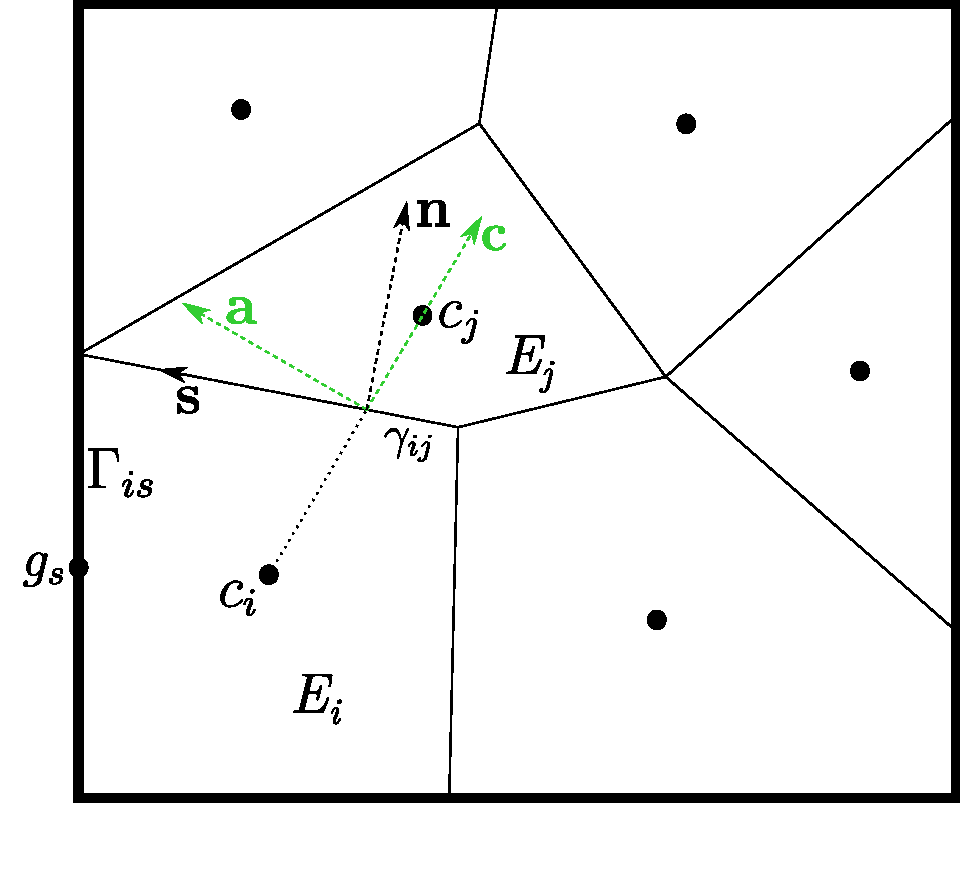
\includegraphics[width=0.4\linewidth]{fvm_grid.pdf}
\caption{Конечнообъёмная сетка}
\label{fig:fvm_grid}
\end{figure}

Проинтегрируем исходное уравнение
по одной из подобластей $E_i$:
\begin{equation*}
-\arint{\nabla^2 u}{E_i}{s} = \arint{f}{E_i}{\vec x}.
\end{equation*}
К интегралу в левой части применим формулу интегрирования по частям \cref{eq:partint_laplace}. Получим
\begin{equation}
\label{eq:fvm_pois_int}
-\arint{\dfr{u}{n}}{\partial E_i}{s} = \arint{f}{E_i}{\vec x}.
\end{equation}
Здесь $\partial E_i$ -- совокупность всех границ подобласти $E_i$,
а $\vec n$ -- внешняя к подобласти нормаль.

Граница ячейки $E_i$ состоит из внутренних граней $\gamma_{ij}$ (индекс $j$ здесь
соответствует индексу соседней ячейки)
и граней $\Gamma_{is}$, лежащих на внешней границе расчётной области $D$.
Тогда интеграл по общей границе ячейки распишется через сумму интегралов по плоским поверхностям
$$
\arint{\dfr{u}{n}}{\partial E_i}{s} = \sum_j\arint{\dfr{u}{n}}{\gamma_{ij}}{s} + \sum_s\arint{\dfr{u}{n}}{\Gamma_{is}}{s}.
$$
Аппроксимирум производную $\dsfr{u}{n}$ на каждой из граней константой.
Тогда её можно вынести из под интегралов и предыдущее выражение записать в виде
\begin{equation}
\label{eq:fvm_gamma_integral}
\arint{\dfr{u}{n}}{\partial E_i}{s} \approx
\sum_j
    \left|
        \gamma_{ij}
    \right|
    \left(
        \dfr{u}{n}
    \right)_{\gamma_{ij}}
+\sum_s
    \left|
        \Gamma_{is}
    \right|
    \left(
        \dfr{u}{n}
    \right)_{\Gamma_{is}}
\end{equation}

Аналогично, анализируя интеграл правой части \cref{eq:fvm_pois_int},
приблизим значение функции правой части $f$ внутри элемента $E_i$ константой $f_i$,
которую отнесём к центру элемента. Тогда
\begin{equation}
\label{eq:fvm_f_integral}
\arint{f}{E_i}{\vec x} \approx f_i \left|E_i\right|.
\end{equation}

\subsubsubsection{Обработка внутренних граней}
Рассмотрим значение нормальной производной по грани $\gamma_{ij}$,
входящее в первое слагаемое правой части \cref{eq:fvm_gamma_integral}.
Для двумерного случая распишем градиент $u$ в системе координат,
образованной еодиничными векторами нормали $\vec n$ и касательной $\vec s = (-n_y, n_x)$
к грани $\gamma_{ij}$:
$$
\nabla u = \dfr{u}{n}\vec n + \dfr{u}{s} \vec s.
$$
Теперь введём другую систему координат, которая образована
векторами $\vec c$ -- нормированный вектор $\vec c_j - \vec c_i$
и перпендикулярного к нему единичного вектора $\vec c^\perp = \vec a = (-c_y, c_x)$
(см. зелёные вектора на \figref{fig:fvm_grid}).
В этой системе
$$
\nabla u = \dfr{u}{c}\vec c + \dfr{u}{a} \vec a.
$$
Пользуясь формулами поворота систем координат $(\vec c, \vec a) \to (\vec n, \vec s)$
искомую производную можно записать
\begin{equation}
\label{eq:fvm_dudn_mult}
\dfr{u}{n} = \dfr{u}{c} \cos(\vecangle{c}{n}) + \dfr{u}{a} \sin(\vecangle{c}{n}).
\end{equation}
Можно рассмотреть и обратный поворот $(\vec n, \vec s) \to (\vec c, \vec a)$:
$$
\dfr{u}{c} = \dfr{u}{n} \cos(\vecangle{n}{c}) + \dfr{u}{s} \sin(\vecangle{n}{c}).
$$
Тогда
\begin{equation}
\label{eq:fvm_dudn_div}
\dfr{u}{n} = \dfr{u}{c} \frac{1}{\cos(\vecangle{n}{c})} - \dfr{u}{s} \tan(\vecangle{n}{c}).
\end{equation}
Таким образом, мы получили два соотношения для определения производной $\dsfr{u}{n}$: \cref{eq:fvm_dudn_mult}, \cref{eq:fvm_dudn_div}.

Отметим, что в трёхмерном случае эти формулы так же остаются справедливыми.
При этом векторы $\vec s$ и $\vec a$ следует строить в плоскости, образованной векторами $\vec n$ и $\vec c$:
\begin{equation*}
\vec s = \frac{\left(\vec n \times \vec c\right) \times \vec n}{\left|\left(\vec n \times \vec c\right) \times \vec n\right|}, \quad
\vec a = \frac{\left(\vec n \times \vec c\right) \times \vec c}{\left|\left(\vec n \times \vec c\right) \times \vec c\right|}.
\end{equation*}
При выводе этих формул используется тот факт, что результат векторного произведения перпендикулярено плоскости, образованной его аргументами.

Определим значения функции $u$ в точках $c_i$, $c_j$ как $u_i$, $u_j$.
Тогда входящая в оба соотношения \cref{eq:fvm_dudn_mult,eq:fvm_dudn_div} производная $\dsfr{u}{c}$ 
может быть приближена конечной разностью
$$
\dfr{u}{c} \approx \frac{u_j - u_i}{|\vec c_j - \vec c_i|}.
$$

Вторые слагаемые в правых частях \cref{eq:fvm_dudn_mult,eq:fvm_dudn_div} можно в первом приближении отбросить, если считать, что угол между векторами $\vec c$ и $\vec n$ 
близок к нулю: $\vecangle{n}{c} \approx 0$.
Тогда искомую производную можно записать в виде:
\begin{equation}
\label{eq:fvm_dudn_approx}
\dfr{u}{n} \approx \frac{u_j - u_i}{h_{ij}},
\end{equation}
где эффективное расстояние $h_{ij}$ между узлами $c_j$ и $c_i$ для приближения \cref{eq:fvm_dudn_mult} запишется как
\begin{equation}
\label{eq:fvm_hij_mult}
h_{ij} = \frac{|\vec c_j - \vec c_i|}{\cos(\vecangle{n}{c})} = \frac{|\vec c_j - \vec c_i|^2}{(\vec c_j - \vec c_i)\cdot \vec n}.
\end{equation}
а для \cref{eq:fvm_dudn_div} --
\begin{equation}
\label{eq:fvm_hij_div}
h_{ij} = |\vec c_j - \vec c_i|\cos(\vecangle{n}{c}) = (\vec c_j - \vec c_i)\cdot \vec n
\end{equation}
Здесь для упрощений было использовано соотношение $\vec a \cdot \vec b = |\vec a||\vec b|\cos(\vecangle{a}{b})$
и единичная длина вектора нормали: $|\vec n| = 1$.

Если вектора $\vec c$ и $\vec n$ сонаправлены, то $\cos(\vecangle{n}{c})=0$ и тогда
формулы \cref{eq:fvm_hij_mult,eq:fvm_hij_div} идентичны.
Если же при этом равны и расстояния от точек $c_j$, $c_i$ до
границы $\gamma_{ij}$, то конечная разность \cref{eq:fvm_dudn_approx}
является симметричной и поэтому имеет второй порядок аппроксимации.
Сетки, которые сохраняют такие свойства, называются
pebi-сетками (perpendicular bisector). Строятся такие сетки на основе ячеек Вороного.


Для сильно скошенных сеток кажется, что использование
формулы \cref{eq:fvm_hij_mult} безопаснее чем \cref{eq:fvm_hij_div}.
Потому что отброшенное из формулы \cref{eq:fvm_dudn_div} 
слагаемое 
$$
\dfr{u}{s}\tan(\vecangle{n}{c})
$$
стремится к бесконечности в вырожденном случае $\vecangle{n}{c} \to \tfrac{\pi}{2}$.
Однако следует понимать, что обе эти формулы
имеют одинаковый первый порядок точности
(это следует из разложения синуса и тангенса вокруг нуля).

\subsubsubsection{Учёт граничных условий}
Для вычисления второго слагаемого в правой части 
\cref{eq:fvm_gamma_integral}
следует расписать значение нормальной 
к границе производной вида
$$
\left(\dfr{u}{n}\right)_{\Gamma_{is}}.
$$
Это делается с помощью граничных условий.
Далее рассмотрим постановку трёх видов граничных условий.

\paragraph{Граничные условия первого рода}
Пусть на центре грани $\Gamma_{is}$ задано 
значение искомой функции
\begin{equation*}
\vec x \in \Gamma_{is}: \quad u(\vec x) = u^\Gamma.
\end{equation*}
Аппроксимацию производных
будем проводить из тех же соображений, которые использовали
при анализе внутренних граней. Только вместо центра соседнего элемента
$c_j$ будем использовать центр грани $g_s$.
В первом приближении, отбрасывая касательные производные, придём к формуле аналигичной \cref{eq:fvm_dudn_approx}:
\begin{equation}
\label{eq:fvm_bc1_approx}
\dfr{u}{n} \approx \frac{u^\Gamma - u_i}{h_{is}},
\end{equation}
где эффективное расстояние $h_{is}$ зависимости от использованного подхода \cref{eq:fvm_dudn_mult} или \cref{eq:fvm_dudn_div}
вычисляется по одному из соотношений
\begin{align}
\label{eq:fvm_dudn_bc_mult}
&h_{is} = \frac{|\vec g_s - \vec c_i|^2}{(\vec g_s - \vec c_i)\cdot \vec n},
\\[10pt]
\label{eq:fvm_dudn_bc_div}
&h_{is} = (\vec g_s - \vec c_i)\cdot \vec n.
\end{align}

\paragraph{Граничные условия второго рода}
Учёт условий второго рода тривиален.
Если на центре грани $\Gamma_{is}$ задано 
значение нормальной производной
\begin{equation}
\label{eq:fvm_bc2_approx}
\vec x \in \Gamma_{is}: \quad \dfr{u}{n} = q,
\end{equation}
то это значение просто подставляется вместо соответствующей производной
в  \cref{eq:fvm_gamma_integral}.

\paragraph{Граничные условия третьего рода}
Теперь рассмотрим условия третьего рода
\begin{equation*}
\vec x \in \Gamma_{is}: \quad \dfr{u}{n} = \alpha u + \beta.
\end{equation*}
Распишем производную в форме \cref{eq:fvm_bc1_approx}:
$$
\frac{u^\Gamma - u_i}{h_{is}} = \alpha u^\Gamma + \beta,
$$
откуда выразим $u^\Gamma$:
$$
u^\Gamma =  \frac{u_i + \beta h_{is}}{1 - \alpha h_{is}}.
$$
Подставляя это выражение в исходное граничное условие получим
\begin{equation}
\label{eq:fvm_bc3_approx}
\dfr{u}{n} \approx \frac{\alpha}{1 - \alpha h_{is}} u_i + \frac{\beta}{1 - \alpha h_{is}}.
\end{equation}

\subsubsection{Одномерный случай}
Рассмотрим результат конечнообъёмной аппроксимации
задачи \cref{eq:fvm_pois} в одномерном случае
на равномерной сетке с шагом $h$ (\figref{fig:fvm_grid1d}).

\begin{figure}[h!]
\centering
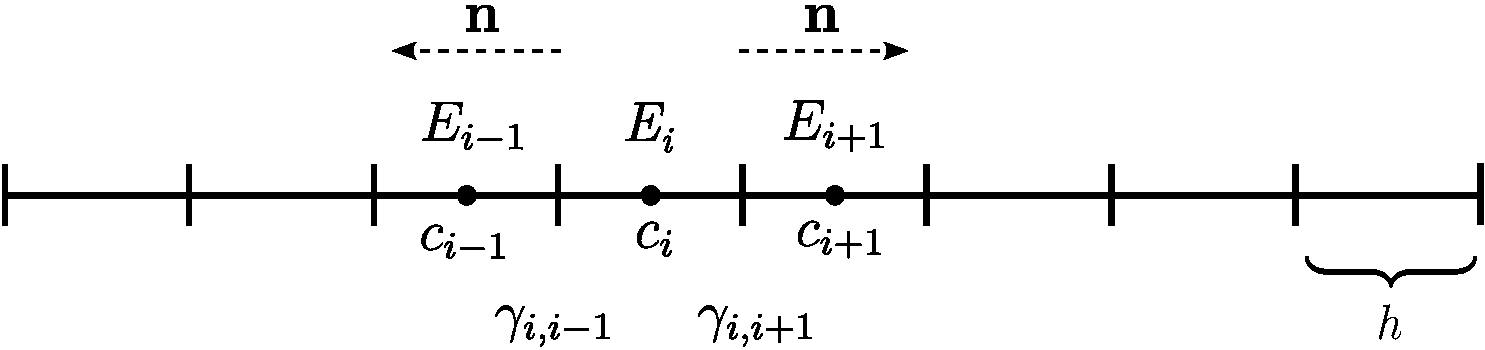
\includegraphics[width=0.6\linewidth]{fvm_grid1d.pdf}
\caption{Одномерная конечнообъёмная сетка}
\label{fig:fvm_grid1d}
\end{figure}

У внутренней ячейки $i$ есть две границы: $\gamma_{i,i-1}$ и $\gamma_{i,i+1}$.
Нормали по этим границам аппроксимируются по формулам \cref{eq:fvm_dudn_approx}:
\begin{align*}
\gamma_{i,i-1}: \quad& \dfr{u}{n} = \frac{u_{i-1}-u_{i}}{h} \\[10pt]
\gamma_{i,i+1}: \quad& \dfr{u}{n} = \frac{u_{i+1}-u_{i}}{h}
\end{align*}
Объём ячейки в одномерном случае равен её длине $h$.
Площадь грани следует положить единице с тем, чтобы
$$
|E_i| = |\gamma| h = h.
$$
Тогда, подставляя эти значения в \cref{eq:fvm_pois_int},
получим знакомую конечноразностную схему аппроксимацию уравнения Пуассона
$$
\frac{-u_{i-1} + 2 u_i - u_{i+1}}{h} = f_i h,
$$
которая имеет второй порядок точности.
Разница с методом конечных разностей здесь состоит в том,
что значения сеточных векторов $\gvec{u}$, $\gvec{f}$ здесь
приписаны к центрам ячеек, а не к их узлам.
Это отличие проявит себя в аппроксимации граничных условий.
Так, если на левой границе задано условие первого рода, то соответствующее уравнение
согласно \cref{eq:fvm_bc1_approx}
примет вид
$$
-\frac{u^\Gamma - u_0}{h/2} - \frac{u_1 - u_0}{h} = f_0 h.
$$
В методе конечных разностей это условие выразилось бы в виде $u_0 = u^\Gamma$.

\subsubsection{Сборка системы линейных уравнений}
Подставим все полученные аппроксимации
\cref{eq:fvm_dudn_approx,eq:fvm_bc1_approx,eq:fvm_bc2_approx,eq:fvm_bc3_approx}
в уравнение \cref{eq:fvm_pois_int}:
\begin{equation*}
-\sum_j
    \frac{|\gamma_{ij}|}{h_{ij}}
         \left(u_j - u_i\right)
-\sum_{s\in{\rm I}}
    \frac{|\Gamma_{is}|}{h_{is}}
        \left(u^\Gamma - u_i\right)
-\sum_{s\in{\rm II}}
    |\Gamma_{is}| q
-\sum_{s\in{\rm III}}
    \frac{|\Gamma_{is}|}{1 - \alpha h_{is}}
    \left(\alpha u_i + \beta\right)
=
f_i |E_i|.
\end{equation*}
Здесь первое слагаемое в левой части отвечает за потоки через внутренние границы,
второе -- граничные условия первого рода, третье -- граничные условия второго рода
и четвёртое -- граничные условия третьего рода.
Далее перенесём все известные значения в правую часть и окончательно
получим линейное уравнение для $i$-го конечного объёма:
\begin{equation}
\label{eq:fvm_slae}
\begin{split}
&\sum_j
    \frac{|\gamma_{ij}|}{h_{ij}}
         \left(u_i - u_j\right)
+\sum_{s\in{\rm I}}
    \frac{|\Gamma_{is}|}{h_{is}}u_i
-\sum_{s\in{\rm III}}
    \frac{\alpha |\Gamma_{is}|}{1 - \alpha h_{is}}
    u_i 
\\[10pt]
&\qquad =
f_i |E_i|
+\sum_{s\in{\rm I}}
    \frac{|\Gamma_{is}|}{h_{is}} u^\Gamma
+\sum_{s\in{\rm II}}
    |\Gamma_{is}| q
+\sum_{s\in{\rm III}}
    \frac{\beta |\Gamma_{is}|}{1 - \alpha h_{is}}.
\end{split}
\end{equation}
Таким образом мы получили систему из $N$ (по количеству подобластей) линейных уравнений относительно
неизвестного сеточного вектора $\left\{u_i\right\}$
$$
A u = b.
$$

\subsubsubsection{Алгоритм сборки в цикле по ячейкам}
Матрицу $A$ и правую часть $b$ системы \cref{eq:fvm_slae} можно
собирать в цикле по ячейкам: строчка за строчкой.
Такой алгоритм выглядел бы следующим образом
\begin{equation*}
\begin{array}{ll}
\textbf{for } i = \overline{0, N-1}                          & \textrm{-- цикл по строкам СЛАУ}\\
\qquad b_i = |E_i| f_i                                       & \\
\qquad \textbf{for } j \in \textrm{nei(i)}                   & \textrm{-- цикл по ячейкам, соседним с ячейкой $i$}\\
\qquad \qquad v = \sfrac{|\gamma_{ij}|}{h_{ij}}              & \\
\qquad \qquad A_{ii} \pluseq v                               & \\
\qquad \qquad A_{ij} \minuseq v                              & \\
\qquad \textbf{endfor}                                       & \\
\qquad \textbf{for } s \in \textrm{bnd1(i)}                  & \textrm{-- цикл по граням ячейки $i$ с условиями первого рода}\\
\qquad \qquad v = \sfrac{|\Gamma_{is}|}{h_{is}}              & \\
\qquad \qquad A_{ii} \pluseq v                               & \\
\qquad \qquad b_{i}  \pluseq u^{\Gamma} v                    & \\
\qquad \textbf{endfor}                                       & \\
\qquad \textbf{for } s \in \textrm{bnd2(i)}                  & \textrm{-- цикл по граням ячейки $i$ с условиями второго рода}\\
\qquad \qquad b_{i}  \pluseq q |\Gamma_{is}|                 & \\
\qquad \textbf{endfor}                                       & \\
\qquad \textbf{for } s \in \textrm{bnd3(i)}                  & \textrm{-- цикл по граням ячейки $i$ с условиями третьего рода}\\
\qquad \qquad v = \sfrac{|\Gamma_{is}|}{(1 - \alpha h_{is})} & \\
\qquad \qquad A_{ii} \minuseq \alpha v                       & \\
\qquad \qquad b_{i}  \pluseq \beta v                         & \\
\qquad \textbf{endfor}                                       & \\
\textbf{endfor}
\end{array}
\end{equation*}
Первым недостатком такого алгоритма является наличие вложенных циклов.
Во-вторых, коэффициент, отвечающий за поток через внутреннюю грань $\gamma_{ij}$,
равный $\sfrac{|\gamma_{ij}|}{h_{ij}}$ в таком алгоритме будет учитывваться дважды:
в строке $i$ и в строке $j$.

\subsubsubsection{Алгоритм сборки в цикле по граням}
Вместо общего цикла по ячейкам, будем использовать цикл по граням.
В таком цикле коэффициенты потоков будут вычисляться один раз
и вставляться сразу в две строки матрицы, соответствующие соседним с гранью ячейкам.
Вложенных циклов в такой постановке удаётся избежать, потому
что у грани есть только две соседние ячейки (в то время как у ячейки может быть произвольное
количество соседних граней).

Разделим все грани на исходной сетки на внутренние и граничные (отдельный набор для каждого вида граничных условий).
Тогда для внутренних граней можно записать
\begin{equation}
\label{eq:fvm_assem_internal}
\begin{array}{ll}
\textbf{for } s \in\textrm{internal}                     & \textrm{-- цикл по внутренним граням}\\ 
\qquad i,j = \textrm{nei\_cells(s)}                      & \textrm{-- две ячейки, соседние с текущей гранью}\\
\qquad v = \sfrac{|\gamma_{ij}|}{h_{ij}}                 & \\
\qquad A_{ii} \pluseq  v; \quad A_{jj} \pluseq  v        & \textrm{-- диагональные коэффициенты матрицы}\\ 
\qquad A_{ij} \minuseq v; \quad A_{ji} \minuseq v        & \textrm{-- внедиагональные коэффициенты матрицы}\\
\textbf{endfor}                                          & \\
\end{array}
\end{equation}
Граничные условия учитываются в отдельных циклах.
Здесь будем учитывать, что у грани, принадлежащей
границе области, есть только одна соседняя ячейка.
Условия первого рода:
\begin{equation}
\label{eq:fvm_assem_bc1}
\begin{array}{ll}
\textbf{for } s \in\textrm{bnd1}                         & \textrm{-- грани с условиями первого рода}\\ 
\qquad i = \textrm{nei\_cells(s)}                        & \textrm{-- соседняя с граничной гранью ячейка}\\
\qquad v = \sfrac{|\Gamma_{is}|}{h_{is}}                 & \\
\qquad A_{ii} \pluseq  v                                 & \\ 
\qquad b_{i} \pluseq u^\Gamma v                          & \\
\textbf{endfor}                                          & \\
\end{array}
\end{equation}
Условия второго рода:
\begin{equation}
\label{eq:fvm_assem_bc2}
\begin{array}{ll}
\textbf{for } s \in\textrm{bnd2}                         & \textrm{-- грани с условиями второго рода}\\ 
\qquad i = \textrm{nei\_cells(s)}                        & \textrm{-- соседняя с граничной гранью ячейка}\\
\qquad b_{i} \pluseq |\Gamma_{is}| q                     & \\
\textbf{endfor}                                          & \\
\end{array}
\end{equation}
Условия третьего рода:
\begin{equation}
\label{eq:fvm_assem_bc3}
\begin{array}{ll}
\textbf{for } s \in\textrm{bnd3}                         & \textrm{-- грани с условиями третьего рода}\\ 
\qquad i = \textrm{nei\_cells(s)}                        & \textrm{-- соседняя с граничной гранью ячейка}\\
\qquad v = \sfrac{|\Gamma_{is}|}{(1 + \alpha h_{is})}    & \\
\qquad A_{ii} \minuseq  \alpha v                         &\\ 
\qquad b_{i} \pluseq \beta v                             & \\
\textbf{endfor}                                          &
\end{array}
\end{equation}
Первое слагаемое в правой части
\cref{eq:fvm_slae}
учтём отдельным циклом:
\begin{equation}
\label{eq:fvm_assem_f}
\begin{array}{ll}                                         & \\
\textbf{for } i = \overline{0,N-1}                        & \textrm{-- цикл по ячейкам}\\ 
\qquad b_i = |E_i| f_i                                    & \\
\textbf{endfor}                                           &
\end{array}
\end{equation}

\subsection{Работа с конечнообъёмной сеткой}
\label{sec:fvm-grid-algos}
Конечнообъёмная сетка разбивает область решения $D$ на непересекающиеся подобласти (ячейки) $E_i$
с плоскими гранями. Выпуклость каждой из подобластей математически не требуется,
но желательна для качественной аппроксимации нормальных производных через грань.
Для ячеек, узлов и граней сетки вводится нумерация. 

Для реализации сборки системы линейных уравнений по 
алгоритму \cref{eq:fvm_assem_internal,eq:fvm_assem_bc1,eq:fvm_assem_bc2,eq:fvm_assem_bc3,eq:fvm_assem_f}
необходимо уметь вычислять следующие параметры конечнообъёмной сетки:
\begin{itemize}
\item
таблица связности грань-ячейка
\item
объём ячейки
\item
центр ячейки
\item
площадь грани
\item
центр грани
\item
нормаль к грани.
\end{itemize}

\subsubsection{Двумерная сетка}

\begin{figure}[h!]
\centering
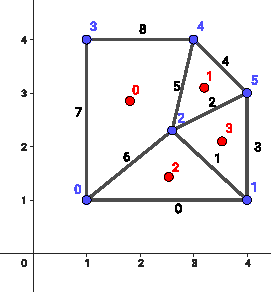
\includegraphics[width=0.4\linewidth]{fvm-mesh-2d.pdf}
\caption{Двумерная конечнообъёмная сетка. Нумерация узлов (синим), ячеек (красным) и граней (чёрным)}
\label{fig:fvm-mesh-2d}
\end{figure}

\subsubsubsection{Определение двумерной конечнообъёмной сетки}
Подобласти представляют собой полигоны с произвольным количеством узлов.
Для однозначного задания такой сетки достаточно таблицы с координатами узлов и таблицы, определяющей ячейки как
последовательности узлов против часовой стрелки (таблица связности \quo{ячейка--узел}).
Для сетки, представленной на \figref{fig:fvm-mesh-2d} эти таблицы будут иметь вид, представленный в 
таблицах \ref{tab:fvm_tab_point}, \ref{tab:fvm_tab_cell_point}.
\begin{table}[H]
\begin{center}
  \begin{minipage}[t]{.4\textwidth}
    \begin{tabular}[t]{c|c|c}
    Узел & X & Y \\
    \hline
    0 & 1 & 1 \\
    1 & 4 & 1 \\
    2 & 2.6 & 2.3 \\
    3 & 1 & 4 \\
    4 & 3 & 4 \\
    5 & 4 & 3 \\
    \end{tabular}
    \caption{\label{tab:fvm_tab_point}Таблица узлов}
  \end{minipage}%
  \quad
  \begin{minipage}[t]{.4\textwidth}
    \begin{tabular}[t]{c|l}
    Ячейка & Узлы \\
    \hline
    0 &  0 2 4 3\\
    1 &  2 5 4\\
    2 &  0 1 2\\
    3 &  1 5 2\\
    \end{tabular}
    \caption{\label{tab:fvm_tab_cell_point}Таблица \quo{ячейка--узел}}
  \end{minipage}
\end{center}
\end{table}

\subsubsubsection{Вспомогательные таблицы связности}

На основании таблицы \quo{ячейка--узел} можно собрать все присутсвующие в сетке
грани в таблицу связности \quo{грань-узел} (см. таблицу \ref{tab:fvm_tab_face_point}).
Направление отрезка границы здесь выбирается произвольно.

\begin{table}[H]
\begin{center}
\begin{tabular}{c|c|c}
Грань & Начальный узел & Конечный узел \\
\hline
0 &  0 & 1\\
1 &  1 & 2\\
2 &  2 & 5\\
3 &  1 & 5\\
4 &  4 & 5\\
5 &  2 & 4\\
6 &  0 & 2\\
7 &  0 & 3\\
8 &  3 & 4\\
\end{tabular}
\caption{\label{tab:fvm_tab_face_point}Таблица связности \quo{грань--узел}}
\end{center}
\end{table}

Так же необходимо собрать таблицу связности \quo{грань-ячейка} (таблица \ref{tab:fvm_tab_face_cell}). Очевидно,
у внутренних граней будет две соседние ячейки, а у граничных -- одна.
При сборке этой таблицы будем учитывать направление отрезка грани. На первую
позицию будем помещать ячейку, расположенную справа от отрезка, а на вторую -- слева.
Первую позицию будем называть отрицательной стороной (поскольку она расположена против направления
нормали к этой грани), а вторую -- положительной.
Если с какой-то из сторон ячейка отсутствует (для граничных граней),
то на соответсвующее место поставим невалидный индекс (в зависимости от реализации это может быть $-1$, максимальное положительное число и т.п.).
Наличие невалидного индекса в таблице \quo{грань-ячейка} можно использовать для выделения граничных граней.

\begin{table}[H]
\begin{center}
\begin{tabular}{c|c|c}
Грань & \makecell{Ячейка справа \\ (отрицательная)} & \makecell{Ячейка слева \\ (положительная)}\\
\hline
0 &  -- & 2  \\
1 &  3  & 2  \\
2 &  3  & 1  \\
3 &  -- & 3  \\
4 &  1  & -- \\
5 &  1  & 0  \\
6 &  2  & 0  \\
7 &  0  & -- \\
8 &  0  & -- \\
\end{tabular}
\caption{\label{tab:fvm_tab_face_cell}Таблица связности \quo{грань--ячейка}}
\end{center}
\end{table}

\subsubsubsection{Геометрические свойства сетки}
После определения всех связной, можно приступить к вычислению геометрических
параметров сетки. На основании таблицы узлов (таб.~\ref{tab:fvm_tab_point}) и таблицы \quo{грань-узел} (таб.~\ref{tab:fvm_tab_face_point})
вычислим площади граней $|\gamma|$ (в двумерном случае площадь грани -- есть длина отрезка грани)
по формуле
$$
|\gamma| = \sqrt{(x_1-x_0)^2 + (y_1 - y_0)^2},
$$
где $x_{0,1}, y_{0,1}$ -- кординаты начальной и конечной точек отрезка грани (таб.~\ref{tab:fvm_tab_face_area}).
Центр грани $\vec g$ (таб.~\ref{tab:fvm_tab_face_center}) определяется как геометрический центр соответствующего отрезка
$$
g_x = \frac{x_0 + x_1}2, \qquad g_y = \frac{y_0 + y_1}2.
$$
Вектор единичной нормали к граням $\vec n$ (таб.~\ref{tab:fvm_tab_face_normal}),
смотрящий влево от направленного отрезка грани, вычисляется по формуле
$$
n_x = -\frac{y_1 - y_0}{|\gamma|}, \qquad n_y = \frac{x_1 - x_0}{|\gamma|}.
$$

\begin{table}[H]
\centering
    \begin{minipage}[t]{.3\linewidth}
        \centering
        \begin{tabular}[t]{c|l}
        Грань & Площадь\\
        \hline
        0 &  3      \\
        1 &  1.91   \\
        2 &  1.57   \\
        3 &  2      \\
        4 &  1.41   \\
        5 &  1.75   \\
        6 &  2.06   \\
        7 &  3      \\
        8 &  2      \\
        \end{tabular}
        \caption{\label{tab:fvm_tab_face_area} Площадь граней}
    \end{minipage}
    \;
    \begin{minipage}[t]{.3\linewidth}
        \centering
        \begin{tabular}[t]{c|l|l}
        Грань & $g_x$ & $g_y$ \\
        \hline
        0 &  2.5    &  1    \\
        1 &  3.3    &  1.65 \\
        2 &  3.3    &  2.65 \\
        3 &  4      &  2    \\
        4 &  3.5    &  3.5  \\
        5 &  2.8    &  3.15 \\
        6 &  1.8    &  1.65 \\
        7 &  1      &  2.5  \\
        8 &  2      &  4    \\
        \end{tabular}
        \caption{\label{tab:fvm_tab_face_center} Центр граней}
    \end{minipage}
    \;
    \begin{minipage}[t]{.3\linewidth}
      \centering
      \begin{tabular}[t]{c|l|l}
      Грань & $n_x$ & $n_y$ \\
      \hline
        0 & $ 0   $   & $ 1   $ \\
        1 & $-0.68$   & $-0.73$ \\
        2 & $-0.45$   & $ 0.89$ \\
        3 & $-1   $   & $ 0   $ \\
        4 & $ 0.71$   & $ 0.71$ \\
        5 & $-0.97$   & $ 0.23$ \\
        6 & $-0.63$   & $ 0.78$ \\
        7 & $-1   $   & $ 0   $ \\
        8 & $ 0   $   & $ 1   $ \\
      \end{tabular}
      \caption{\label{tab:fvm_tab_face_normal} Нормаль к граням}
    \end{minipage}
\end{table}

Для вычисления объёмов (площадей) (таб.~\ref{tab:fvm_tab_cell_volume}) и центров масс (таб.~\ref{tab:fvm_tab_cell_center}) ячеек воспользуемся таблицей \quo{ячейка-узел},
где задана нумерация узлов ячеек против часовой стрелки.
Алгоритмы вычисления представлены в пп.~\ref{sec:polygon_area}, ~\ref{sec:polygon_center}.
\begin{table}[H]
\centering
    \begin{minipage}[t]{.4\linewidth}
      \centering
      \begin{tabular}[t]{c|l}
      Ячейка & Объём\\
      \hline
      0 &  4.1    \\
      1 &  1.05   \\
      2 &  1.95   \\
      3 &  1.4    \\
      \end{tabular}
      \caption{\label{tab:fvm_tab_cell_volume} Объём ячеек}
    \end{minipage}
    \qquad
    \begin{minipage}[t]{.4\linewidth}
        \centering
        \begin{tabular}[t]{c|l|l}
        Ячейка & Центр X & Центр Y \\
        \hline
        0 &  1.81   &  2.85 \\
        1 &  3.2    &  3.1  \\
        2 &  2.53   &  1.43 \\
        3 &  3.53   &  2.1  \\
        \end{tabular}
        \caption{\label{tab:fvm_tab_cell_center} Центр ячеек}
    \end{minipage}
\end{table}

\subsubsection{Трёхмерная сетка}
\begin{figure}[h!]
\centering
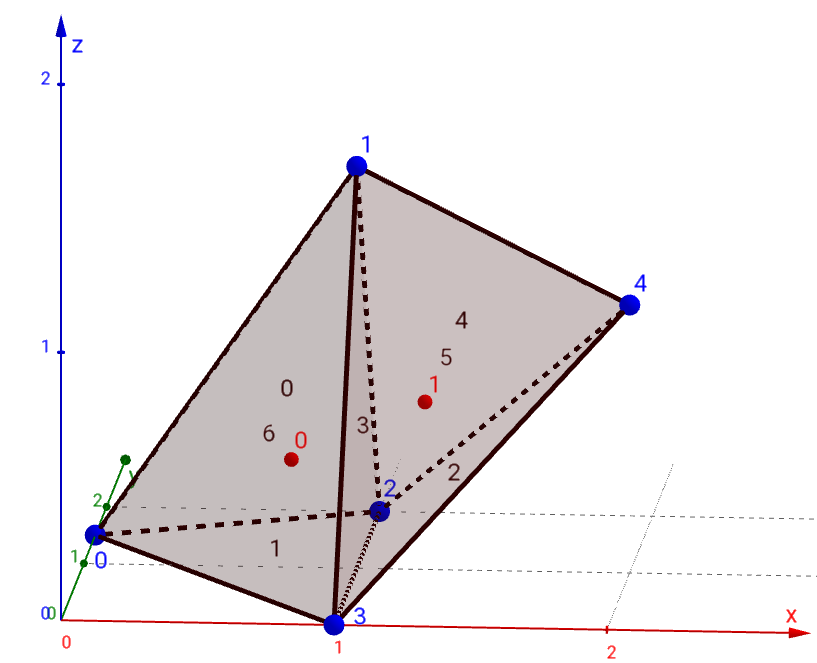
\includegraphics[width=0.45\textwidth]{fvm-mesh-3d-1.png}
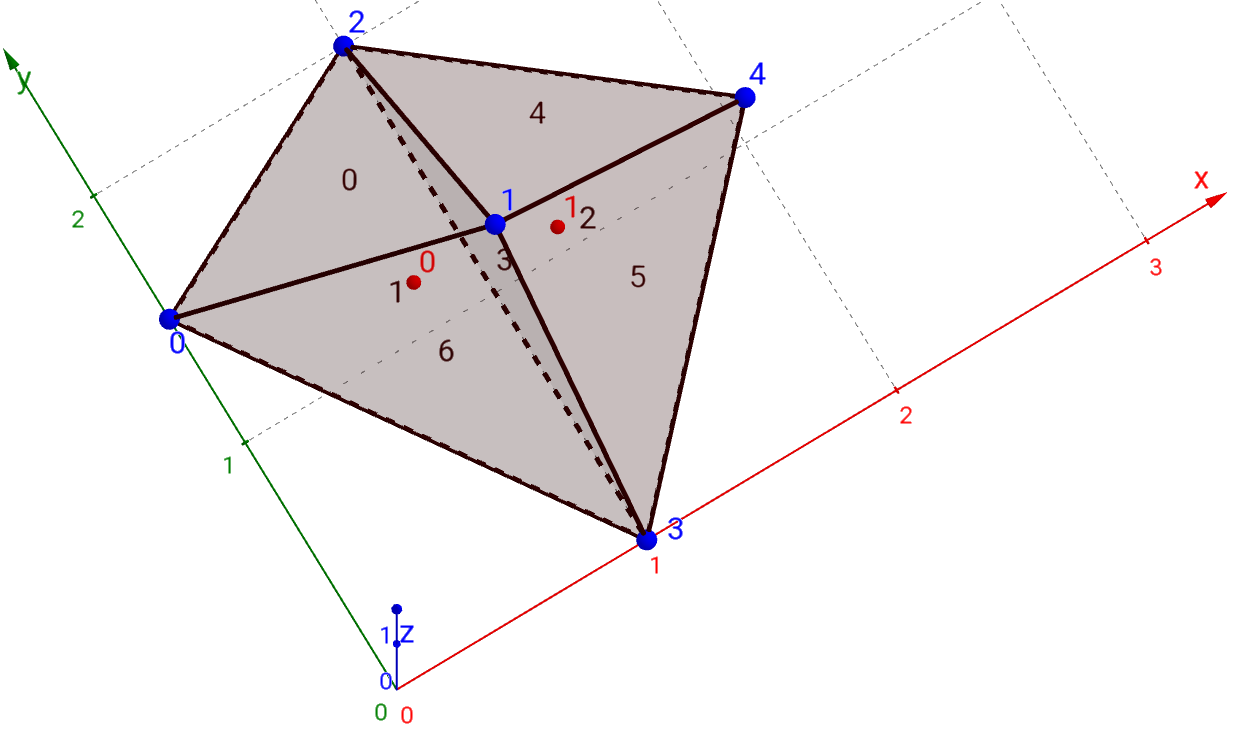
\includegraphics[width=0.54\textwidth]{fvm-mesh-3d-2.png}
\caption{Трёхмерная конечнообъёмная сетка в двух проекциях. Нумерация узлов (синим), ячеек (красным) и граней (чёрным)}
\label{fig:fvm-mesh-2d}
\end{figure}

\subsubsubsection{Определение трёхмерной конечнообъёмной сетки}
Подобласти представляют собой многогранники с произвольным количеством многоугольных граней.
Для примера рассмотрим сетку, представленную на рисунке~\ref{fig:fvm-mesh-2d}.
Чтобы задать такую сетку однозначно, необходимы
\begin{itemize}
\item
таблица узлов (таб.~\ref{tab:fvm3_tab_point});
\item
таблица \quo{грань-узел} (таб.~\ref{tab:fvm3_tab_face_point}), где набор услов задан в последовательном порядке. Направление закрутки здесь произвольное;
\item
таблица \quo{грань-ячейка} (таб.~\ref{tab:fvm3_tab_face_cell}). Порядок задания ячеек зависит от направления закрутки, заданной в предыдущей таблице (\quo{грань-узел}).
Будем смотреть на грань со стороны нормали (с этой стороны обход узлов будет против часовой стрелки).
Тогда на первом месте должна стоять ячейка, находящаяся за плоскостью грани (отрицательная сторона), а на втором -- перед плоскостью грани (положительная сторона).
Если с одной из сторон нет ячейки (для границ), то на это место ставится невалидный индекс.
\end{itemize}

\begin{table}[H]
\begin{center}
  \begin{minipage}[t]{.4\textwidth}
    \centering
    \begin{tabular}[t]{c|c|c|c}
    Узел & X & Y & Z \\
    \hline
    0 & 0   & 1.5 & 0   \\
    1 & 1   & 1   & 1.5 \\
    2 & 1   & 2   & 0   \\
    3 & 1   & 0   & 0   \\
    4 & 2   & 1   & 1   \\
    \end{tabular}
    \caption{\label{tab:fvm3_tab_point}Таблица узлов}
  \end{minipage}%
\end{center}
\end{table}

\begin{table}[H]
\begin{center}
  \begin{minipage}[t]{.4\textwidth}
    \centering
    \begin{tabular}[t]{c|l}
    Грань & Узлы \\
    \hline
    0 & 0 1 2\\
    1 & 0 3 2\\
    2 & 3 2 4\\
    3 & 3 2 1\\
    4 & 2 1 4\\
    5 & 3 4 1\\
    6 & 3 0 1\\
    \end{tabular}
    \caption{\label{tab:fvm3_tab_face_point}Таблица \quo{грань--узел}}
  \end{minipage}%
  \begin{minipage}[t]{.4\textwidth}
    \centering
    \begin{tabular}[t]{c|c|c}
    Грань & \makecell{Ячейка снизу \\ (отрицательная)} & \makecell{Ячейка сверху \\ (положительная) }\\
    \hline
    0 &  0  & --  \\
    1 & --  &  0  \\
    2 &  1  & --  \\
    3 &  0  &  1  \\
    4 &  1  & --  \\
    5 &  1  & --  \\
    6 & --  &  0  \\
    \end{tabular}
    \caption{\label{tab:fvm3_tab_face_cell}Таблица \quo{грань--ячейка}}
  \end{minipage}%
\end{center}
\end{table}

\subsubsubsection{Геометрические свойства сетки}

Площадь (таб.~\ref{tab:fvm3_tab_face_area}) и центр (таб.~\ref{tab:fvm3_tab_face_center})
граней вычисляются согласно алгоритмам из пп.~\ref{sec:polygon_area}, \ref{sec:polygon_center}.
Для определения нормали к плоской грани (таб.~\ref{tab:fvm3_tab_face_normal}) необходимо
взять три последовательные, не лежащие на одной прямой точки
грани из упорядоченной таблицы связности
\quo{грань--узел}:
$\vec{p}_0$, $\vec{p}_1$, $\vec{p}_2$,
и провести векторное умножение:
$$
\vec n = \frac{\vec k}{|\vec k|}, \qquad \vec k = (\vec{p}_1 - \vec{p}_0)\times(\vec{p}_2 - \vec{p}_0).
$$

\begin{table}[H]
\centering
    \begin{minipage}[t]{.3\linewidth}
        \centering
        \begin{tabular}[t]{c|l}
        Грань & Площадь\\
        \hline
        0 &  0.98   \\
        1 &  1      \\
        2 &  1.41   \\
        3 &  1.5    \\
        4 &  0.94   \\
        5 &  0.94   \\
        6 &  1.44   \\
        \end{tabular}
        \caption{\label{tab:fvm3_tab_face_area} Площадь граней}
    \end{minipage}
    \;
    \begin{minipage}[t]{.3\linewidth}
        \centering
        \begin{tabular}[t]{c|l|l|l}
        Грань & $g_x$ & $g_y$ & $g_z$\\
        \hline
        0 & 0.67  & 1.5  & 0.5   \\
        1 & 0.67  & 1.17 & 0     \\
        2 & 1.33  & 1    & 0.33  \\
        3 & 1     & 1    & 0.5   \\
        4 & 1.33  & 1.33 & 0.83  \\
        5 & 1.33  & 0.67 & 0.83  \\
        6 & 0.67  & 0.83 & 0.5   \\
        \end{tabular}
        \caption{\label{tab:fvm3_tab_face_center} Центр граней}
    \end{minipage}
    \;
    \begin{minipage}[t]{.3\linewidth}
      \centering
      \begin{tabular}[t]{c|l|l|l}
      Грань & $n_x$ & $n_y$ & $n_z$ \\
      \hline
        0 & $-0.38$   & $ 0.77$  &  $ 0.51$ \\
        1 & $  0  $   & $  0  $  &  $  1  $ \\
        2 & $ 0.71$   & $  0  $  &  $-0.71$ \\
        3 & $  1  $   & $  0  $  &  $  0  $ \\
        4 & $ 0.27$   & $ 0.8 $  &  $ 0.53$ \\
        5 & $ 0.27$   & $-0.8 $  &  $ 0.53$ \\
        6 & $ 0.78$   & $ 0.52$  &  $-0.35$ \\
      \end{tabular}
      \caption{\label{tab:fvm3_tab_face_normal} Нормаль к граням}
    \end{minipage}
\end{table}

Вычисление объёма (таб.~\ref{tab:fvm3_tab_cell_volume}) и
центра масс (таб.~\ref{tab:fvm3_tab_cell_center}) ячеек
осуществляется по формулам из пп.~\ref{sec:polyhedron_volume}, \ref{sec:polyhedron_center}
соответственно.

\begin{table}[H]
\centering
    \begin{minipage}[t]{.4\linewidth}
      \centering
      \begin{tabular}[t]{c|l}
      Ячейка & Объём\\
      \hline
      0 &  0.5  \\
      1 &  0.5  \\
      \end{tabular}
      \caption{\label{tab:fvm3_tab_cell_volume} Объём ячеек}
    \end{minipage}
    \qquad
    \begin{minipage}[t]{.4\linewidth}
        \centering
        \begin{tabular}[t]{c|l|l|l}
        Ячейка & $c_x$ & $c_y$ & $c_z$ \\
        \hline
        0 &  0.75   &  1.13 & 0.38 \\
        1 &  1.25   &  1    & 0.63 \\
        \end{tabular}
        \caption{\label{tab:fvm3_tab_cell_center} Центр ячеек}
    \end{minipage}
\end{table}


\subsubsection{Интегрирование сеточной функции}
Пусть задана сеточная функция $\gvec{u_i}$, которая аппроксимирует функцию $u$.
Интеграл по области расчёта от этой функции можно расписать через сумму интегралов
по каждой ячейке и далее воспользоваться тем фактом,
что значение аппроксимированной функции внутри ячейки постоянно:
\begin{equation}
\label{eq:fvm_integrate}
\arint{u}{D}{\vec x} = \sum_{i=0}^{N-1} \arint{u}{E_i}{\vec x} \approx \sum_{i=0}^{N-1} u_i |E_i|.
\end{equation}


\subsection{Пример расчётной программы}
\label{sec:prog-poisson2-fvm}

Рассмотрим пример решения двумерного уравнения \cref{eq:fvm_pois}
с граничными условиями первого рода.
Для тестирования методики действовать будем
по аналогии из п.\ref{sec:compute-appr}:
\begin{itemize}
\item
Зададим точное решение в виде
$$
u^e = \cos(10 x^2) \sin(10 y) + \sin(10 x^2)\cos(10 x);
$$
\item
Расчитаем правую часть прямым дифференцированием
$$
f = -\dfrq{u^e}{x} - \dfrq{u^e}{y};
$$
\item
Используя подсчитанную $f$ применим алгоритм метода конечных объёмов для
получения численного решения $u$;
\item
Для вычисления отклонения численного решения от точного подсчитаем интеграл вида
\cref{eq:norm2_common}:
\begin{equation}
\label{eq:fvm_norm2}
||u - u^e||_2 = \sqrt{\frac{1}{D}\arint{\left(u - u^e\right)^2}{D}{\vec x}}.
\end{equation}
\end{itemize}

Пример программы лежит в файле \ename{poisson_fvm_solve_test.cpp}
в тесте \cvar{[]}.
Программа использует регулярную двумерную
сетку в единичном квадрате квадрате с разбиением
в 20 ячеек по каждой оси.
После расчёта файл с численным и точным
решениями сохраняется в файл \ename{poisson2_fvm.vtk},
а на печать выводится количество ячеек в сетке и полученная
норма отклонения. Результат работы программы представлен на \figref{fig:poisson2_fvm}.
Поскольку вектор решений задан в центрах ячеек, то его отображение имеет
мозаичный вид.

\begin{figure}[h!]
\centering
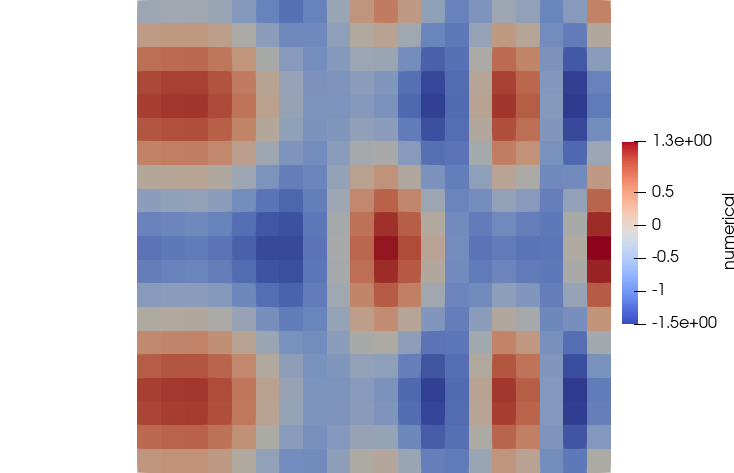
\includegraphics[width=0.5\linewidth]{poisson2_fvm.png}
\caption{Результат расчёта}
\label{fig:poisson2_fvm}
\end{figure}

\subsubsection{Работа с сеткой}
Несмотря на то, что на вход
подаётся регулярная сетка,
все алгоритмы используют сетку
через абстракный интерфейс \cvar{IGrid},
который определён для
сеток произвольной структуры и размерности.
Этот интерфейс (полностью объявленный в файле \ename{grid/i_grid.hpp}) предоставляет следующие функции, используемые в алгоритмах
\cref{eq:fvm_assem_internal,eq:fvm_assem_bc1,eq:fvm_assem_bc2,eq:fvm_assem_bc3,eq:fvm_assem_f}:
\begin{itemize}
\item
\cvar{IGrid::face_normal} -- вектор нормали для заданной грани;
\item
\cvar{IGrid::tab_face_cell} -- таблица связности грань--ячейка. Возвращает
пару индексов ячеек. Первый из этих индексов соответствует ячейке,
лежащией в направлении, противоположенном направлению нормали заданной грани.
Для граничных граней один из этих индексов (в зависимости от направления нормали этой грани)
равен глобальной константе \cvar{INVALID_INDEX};
\item
\cvar{IGrid::face_center} -- центр грани;
\item
\cvar{IGrid::face_area} -- значение площади заданной грани;
\item
\cvar{IGrid::cell_center} -- центр ячейки;
\item
\cvar{IGrid::cell_volume} -- объём ячейки.
\end{itemize}
Конкретная реализация этих функций зависит от вида сетки.
Так, для структурированной сетки \cvar{RegularGrid2D} 
их (тривиальная для таких сеток) реализация 
находится в файле \ename{grid/regular_grid2.cpp}.
Для произвольной двумерной неструктурированной сетки
\cvar{UnstructuredGrid2D}
общие алгоритмы, описанные в пункте \ref{sec:fvm-grid-algos}
реализованы в файле
\ename{grid/unstructured_grid2d.cpp}

\subsubsection{Функция верхнего уровня}
\clisting{open}{"test/poisson_fvm_solve_test.cpp"}
На верхнем уровне создаётся сетка класса \cvar{RegularGrid2D},
которая затем используется при конструировании
робочего класса \cvar{TestPoisson2FvmWorker}.
\clisting{lines-range}{"TEST_CASE", "worker"}
Далее вызывается решатель, который возвращает величину нормы:
\clisting{line}{"solve"}
результат сохраняется в файл
\clisting{line}{"save"}
печатается количество ячеек и полученная норма
\clisting{line}{"cout"}
и полученная норма проверяется с предварительно расчитанным
для заданных параметров значением
\clisting{line}{"CHECK"}

\subsubsection{Инициализация решения}
\clisting{to-start}{}
Рассмотрим рабочий класс \cvar{TestPoisson2FvmWorker}.
В его объявлении реализованы два статических метода:
заданное точное решение
\clisting{block}{"static double exact_solution"}
и подсчитанная правая часть, соответствующая этому решению
\clisting{block}{"static double exact_rhs"}
В полях класса хранятся: ссылка на абстрактную сетку
\clisting{line}{"_grid"}
список внутренних граней
\clisting{line}{"_internal_faces"}
и список граничных граней с условиями первого рода
\clisting{line}{"_dirichlet_faces"}
Каждая из этих граней описана структурой вида
\clisting{to-start}{}
\clisting{block}{"struct DirichletFace"}
в которой хранятся индекс грани,
индекс ячейки, соседней с этой гранью,
граничное значение функции в центре этой грани
и направление внешней к области нормали.

Поле \cvar{_grid} передается в класс пользователем,
в то время как списки \cvar{_internal_faces} и \cvar{_dirichlet_faces}
собираются при конструировании рабочего класса.
\clisting{line}{"TestPoisson2FvmWorker::TestPoisson2FvmWorker(const IGrid& grid)"}
Чтобы отличить внутреннюю грань от граничной, необходимо
проверить таблицу связности грань--ячейка. Если
для грани одно из значений этой таблицы равно \cvar{INVALID_INDEX},
значит с соответствующей стороны нет ячейки, а грань является граничной.
Эта проверка проводится в цикле по граням
\clisting{lines-range}{"for", "icell_positive"}
Если обе ячейки валидны, значит грань внутренняя и её индекс
следует добавить в список \cvar{_internal_faces}
\clisting{lines-range}{"if", "push_back"}
Для граничных граней создаётся и заполняется структура
\cvar{DirichletFace}. Сначала заполняются те поля,
которые не зависят от направления: индекс грани и
граничное значение (которое берётся из точного решения):
\clisting{lines-range}{"DirichletFace", "face_center"}
Далее, если нормаль грани направлена вовне
расчётной области (ячейка по направлению нормали невалида),
то индекс соседней ячейки берётся с отрицательного направления,
а внешняя к области нормаль совпадает с нормалью грани
\clisting{lines-range}{"if", "outer_normal"}
иначе индекс ячейки берётся из положительного направления,
а внешняя к области нормаль противоположна нормали грани
\clisting{block}{"else"}

\subsubsection{Реализация решения}
Решение осуществляется вызовом функции
\clisting{block}{"TestPoisson2FvmWorker::solve()"}
в которой последовательно строятся левая и правая часть СЛАУ,
вызывается решатель СЛАУ и производится сравнение
с точным решением.
\subsubsubsection{Сборка матрицы}
В функции сборки левой части СЛАУ
\clisting{line}{"CsrMatrix TestPoisson2FvmWorker::approximate_lhs()"}
реализуются алгоритмы \cref{eq:fvm_assem_internal,eq:fvm_assem_bc1}
в той их части, которая касается коэффициентов матрицы.
Сначала согласно \cref{eq:fvm_assem_internal}
проходит цикл по внутренним ячейкам
\clisting{line}{"for"}
Для грани берётся нормаль
\clisting{line}{"normal ="}
Вычисляются соседние с гранью ячейки и их центры
\clisting{lines-range}{"negative", "cj ="}
находися эффективное расстояние между ними по модели
\cref{eq:fvm_hij_div}
\clisting{line}{"double h ="}
и далее проводится заполнение матрицы найденным значением потока \cvar{coef}:
\clisting{until-close}{}

Учёт условий первого рода проводится в
цикле по соответствующим граням согласно алгоритму \cref{eq:fvm_assem_bc1}
и модели вычисления эффективного расстояния \cref{eq:fvm_dudn_bc_div}
\clisting{block}{"for"}
 
\subsubsubsection{Сборка правой части}
В сборке правой части
\clisting{lines-range}{"approximate_rhs", "rhs"}
сначала прогоняется алгоритм \cref{eq:fvm_assem_f}
\clisting{block}{"for"}
а затем учитываются граничные условия первого рода согласно \cref{eq:fvm_assem_bc1}
\clisting{block}{"for"}

\subsubsubsection{Вычисление нормы отклонения от точного решения}
Вычисление выражения
\cref{eq:fvm_norm2} с использованием
алгоритма \cref{eq:fvm_integrate}
производится в функции
\clisting{block}{"compute_norm"}

\subsection{Задание для самостоятельной работы}
\label{seq:fvm_poisson_hw}
\paragraph{Получить решения для неструктурированных сеток}
В папке \ename{test_data} корневой директории репозитория
лежат скрипты построения сеток в программе \ename{HybMesh}:
\begin{itemize}
\item \ename{pebigrid.py} -- pebi--сетка,
\item \ename{tetragrid.py} -- сетка, состоящая из произвольных трех- и четырехугольников.
\end{itemize}
Инструкции по запуску этих скриптов смотри п. \ref{sec:hybmesh}.
Эти скрипты строят равномерную неструктурированную сетку
в единичном квадрате
и записывают её в файл vtk, который впоследствии можно загрузить
в расчётную программу.
В каждом из скриптов есть параметр \cvar{N}, означающий
примерное количество ячеек в итоговой сетке.
Меняя его значение можно строить сетки разного разрешения.

Необходимо с помощью этих скиптов построить сетки
из $\sim$1000 ячеек. Далее на этих сетках
решить задачу из п. \ref{sec:prog-poisson2-fvm}
и сравнить поля решений и полученные нормы для этих сеток
и равномерной структурированной сетки сходного разрешения.

Работать на основе теста \cvar{poisson2-fvm}
в файле \ename{poisson2_fvm_solve_test.cpp}.
Можно создать отдельный тест, использующий те же классы для работы.

Для загрузки построенной сетки в решатель необходимо файл
с сеткой поместить в каталог \ename{test_data}
и далее загрузить её в класс \cvar{UnstructuredGrid2D}.
Нижеследующий код прочитает файл \ename{test_data/pebigrid.vtk}
и создаст рабочий класс с использованием прочитанной сетки
\begin{cppcode}
std::string fn = test_directory_file("pebigrid.vtk");
UnstructuredGrid2D grid = UnstructuredGrid2D::vtk_read(fn);
TestPoisson2FvmWorker worker(grid);
\end{cppcode}

\paragraph{Получить порядок аппроксимации}
Для трёх видов сеток: структурированной, pebi и
произвольной  построить график сходимости
аналогичный \figref{fig:poisson_convergence}.
Для этого провести серию расчётов
с различным количеством ячеек в диапазоне $N\in[500, 10^5]$.

Следует иметь ввиду, что на графике сходимости
по оси абсцисс отложено линейное разбиение, вычисляемое как
$n=\sfrac{1}{h}$, где $h$ -- это характерный линейный размер ячейки.
Для неструктурированных двумерных сеток этот линейный размер
сетки можно вычислить через среднюю площадь ячейки $A$ как $h = \sqrt{A}$,
которую в свою очередь можно получить, разделив общую площадь на количество
ячеек: $A = \sfrac{|D|}{N}$.
Тогда, в случае единичного квадрата, линейное разбиение будет равно $n = \sqrt{N}$.

\paragraph{Реализовать граничные условия второго рода}
Решить ту же задачу используя граничные условия второго рода на pebi--сетке
и сравнить полученные результы с решением задачи первого рода.

Для этого нужно в рабочий класс добавить функцию вычисления нормальной производной.
Эта функция будет на вход принимать точку, лежащую на границе единичного квадрата,
и возвращать $\dsfr{u^e}{n}$, вычисленную прямым дифференцированием известного
точного решения. Следует учитывать направление внешней нормали. Например,
на вертикальной границе
\begin{align*}
x=0: \quad &\dfr{u}{n} = -\dfr{u}{x}, \\
x=1: \quad &\dfr{u}{n} = \dfr{u}{x}, \\
\end{align*}
Для определения конкретной границы следует анализировать входную точку.
Поскольку работа ведётся в числах с плавающей точкой, сравнение следует
делать с некоторым допуском:
\begin{cppcode}
struct TestPoisson2FvmWorker{
	// точная производная по x
	static double exact_dudx(Point p){
		...
	}
	// точная производная по y
	static double exact_dudy(Point p){
		...
	}
	static double exact_dudn(Point p){
		double x = p.x();
		double y = p.y();
		if (std::abs(x) < 1e-6){
			// левая граница. Вернуть -du/dx
			return -exact_dudx(p);
		} else if (std::abs(x-1) < 1e-6){
			// правая граница. Вернуть du/dx
			return exact_dudx(p);
		} else if ...
	}
\end{cppcode}

Для реализации алгоритма \cref{eq:fvm_assem_bc2}
предварительно нужно собрать информацию о гранях,
которую следует хранить в массиве структур (по аналогии с \cvar{DirichletFace})
\begin{cppcode}
struct NeumannFace{
	size_t iface;
	size_t icell;
	double value;
};
std::vector<NeumannFace> _neumann_faces;
\end{cppcode}
В отличие от условий Дирихле, структура для условий Неймана не
содержит нормалей, поскольку в формулах \cref{eq:fvm_assem_bc2} они не используются.
Заполнять массив \cvar{_neumann_faces} следует в конструктуре
\cvar{TestPoisson2FvmWorker} вместо \cvar{_dirichlet_faces}.

Алгоритм учёта условий второго рода не изменяет матрицу,
поэтому обработку граничных граней следует убрать
из функции \cvar{approximate_lhs},
а в функции сборки правой части \cvar{approximate_rhs}
нужно реализовать формулы \cref{eq:fvm_assem_bc2}.

Задача в такой постановке имеет бесконечное множество
решений, отличающихся на константу. Для
получения однозначного ответа нужно задать
точное решение в одной из ячеек. Выберем нулевую ячейку.
Тогда нулевое уравнение СЛАУ нужно преобразовать к виду
$$
u_0 = u^e(\vec c_0) \hence A_{0j} = \delta_{0j}, \quad b_0 = u^e(\vec c_0).
$$
Для этого в функции \cvar{approximate_lhs}
после окончания сборки следует вызвать метод
\begin{cppcode}
mat.set_unit_row(0);
\end{cppcode}
а в конце \cvar{approximate_rhs} --
\begin{cppcode}
rhs[0] = exact_solution(_grid.cell_center(0));
\end{cppcode}
